\documentclass[stu, donotrepeattitle, floatsintext, noextraspace, 10pt]{apa7}

\UseRawInputEncoding
\usepackage{hyperref}
\usepackage{booktabs}
\usepackage{longtable}
\usepackage{url}
\usepackage{threeparttable}
\usepackage[american]{babel}
\usepackage{csquotes}
\usepackage{graphicx}
\usepackage{hyperref}
\usepackage{multirow}
\usepackage{caption}
\usepackage{subcaption}
\usepackage{pdflscape}
\usepackage[style=apa, sortcites=true, sorting=nyt, bibencoding=utf8, backend=biber]{biblatex}
\DeclareLanguageMapping{american}{american-apa}
\addbibresource{paper.bib}

\title{Evaluating Automated Redistricting Algorithms Using Measures of Compactness \& Partisan Fairness: A Case Study of 2021 Congressional Redistricting in Virginia}
\authorsnames{{Word Count: 4,987}}
% commented-out to meet AP requirements that there be no identifying info in the paper. 
%\authorsnames{Madeleine Goertz}
\authorsaffiliations{\protect\phantom{International Community School}}
%\authorsaffiliations{$\mspace$}
\course{\protect\phantom{AP Research}}
\professor{\protect\phantom{Randall S. Huberman}}
\duedate{\protect\phantom{May 20th, 2021}}
\authornote{The datasets, source code, and other supplementary materials for this project can be found at \url{https://git.io/JsoZw}.}

\begin{document}
\maketitle

%using input not include so that starts on same page
% Manually putting in the title here and using donotrepeattitle in paper.tex so that I don't have a section header for "Introduction", but there is still a section in the VScode navigation for all the intro subsections to live within. 
\makeatletter
\section{\@title}
\makeatother

Legislative redistricting is the process of drawing district boundaries for elections. In the United States, the redrawing of congressional district boundaries occurs every 10 years after the census. This process of redistricting is generally performed by state legislatures, hybrid commissions, or independent commissions \parencite{princetongerrymanderingproject}. 

When redistricting congressional districts, the two most fundamental requirements are that the districts must be "reasonably compact" and of equal population, meaning that the population of each district must be within $\pm$ 1\% of the average district population \parencite{1964}. 

Gerrymandering means drawing the district boundaries in such a way as to unfairly benefit a particular group, such as a political party or a racial group. There are two primary methods of gerrymandering: "packing" and "cracking." The US Supreme Court defines these as creating districts where the opposing party holds far above the majority or is spread out amongst so many districts as to become ineffectual, respectively \parencite{1986}.

Automated redistricting algorithms are one proposed solution to prevent gerrymandering. As early as 1961, such "automatic and impersonal procedure[s]" were thought to "produce results not markedly inferior to those which would be arrived at by a genuinely disinterested commission" \parencite[110]{vickrey1961}.

Broadly speaking, the goal of such algorithms is to create a map (or a selection of maps) that doesn't distort the will of the people. Some algorithms obey only equal population and compactness constraints \parencite[e.g.][]{hu1995, altman2009, chen2013}, while more-modern algorithms have evolved to address real-world considerations, such as majority-minority districts, incumbency, and competitiveness \parencite[e.g][]{lara-caballero2019, fifield2020, mccartan2020}. 

In parallel to the development of these algorithms, measures of compactness and of partisan fairness were also developed. These compactness measures include geometric measures \parencite[e.g.][]{polsby1991, schwartzberg1966,harris1964, maceachren1985, reock1961, boyce1964} and measures from graph theory \parencite[e.g.][]{dube2016}. Proposed measures of partisan fairness generally try to characterize the relationship between the number of votes and the number of seats won by a political party. Some measures seek to simulate the power balance in the legislature at all possible party votes shares \parencite[e.g.][]{tufte1973}, while others aim to compute a single metric \parencite[e.g.][]{stephanopoulos2014,katz2020,warrington2018,mcdonald2015,wang2016}. Neither the scholarly literature nor the courts agree on a single correct compactness or partisan fairness measure. 

While the scholarship is focused on the development of new automated redistricting algorithms \parencite{fifield2020}, on the evaluation of the mathematical rigor of proposed metrics \parencite[see][]{katz2020}, and on the detection of gerrymandering in existing redistricting plans \parencite[e.g.][]{herschlag2017, duchin2018a}, research into the empirical performance of these algorithms in a real-world redistricting scenario is lacking \parencite{fifield2020a}.

Identifying this gap led me to my research question, \emph{how do the hypothetical district maps for the Virginia Congressional delegation for the 2020s generated by different automated redistricting algorithms compare based on partisan fairness and compactness measures?}

With the goal of comparing the performance of different automated redistricting algorithms, I chose two algorithms of different levels of complexity that could both meet the real-world requirements of equal population and compactness. Since there is no single measure of partisan fairness nor compactness agreed upon by the scholarship, I selected representative samples of the different perspectives on each measure. This research is conducted as a case-study using the experimental research method.

This paper begins with a \hyperref[sec:litreview]{literature review} of the scholarship on automated redistricting algorithms, compactness measures, and partisan fairness measures. Further details of my chosen research method are explained in the \hyperref[sec:method]{Method} section. The results of my analysis are presented, interpreted, and reflected upon in the \hyperref[sec:results]{Results}, \hyperref[sec:disc]{Discussion}, and \hyperref[sec:conc]{Conclusion} sections, respectively. 
\section{Literature Review}
\label{sec:litreview}

I will provide an overview of some of the current research into automated redistricting algorithms and compactness and partisan fairness measures. 

\subsection{Automated Redistricting Algorithms}

The purpose of automated redistricting algorithms is to generate a set of redistricting plans that are as "impartial" as possible \parencite{chen2013}. While many different algorithms have been proposed (see \textcite{altman2009}, \textcite{haas2020}, \textcite{lara-caballero2019}, \textcite{macmillan2001}, \textcite{weaver1963}, and \textcite{xiao2008}), I will provide high-level overviews of two algorithms: \hyperref[sec:smc]{Sequential Monte Carlo (SMC)} and \hyperref[sec:crsg]{Compact Random Seed Growth (CRSG)}. 

\subsubsection{Redistricting as Graph Cutting}
\label{sec:redistasgraphcut}


The following redistricting algorithms, SMC and CRSG, both conceptualize redistricting precincts as a graph-cutting problem. A graph is a network of different interconnected points, where the points are "nodes" and the lines connecting them "edges" \parencite{fifield2020}. Every precinct is a node, and geographically-adjacent precincts have their corresponding nodes connected by edges. This is known as the "adjacency graph." Since the goal of redistricting is to assign every precinct a district, the algorithms imagine that edges between nodes are "cut" until "islands" (known as "subgraphs") are formed, where each is disconnected from the others. The disconnected subgraphs then become the districts. See Figure \ref{fig:graphcut} for a visualization \parencite{fifield2020}. 

\begin{figure}[ht]
    \caption{Redistricting as Graph Cutting}
    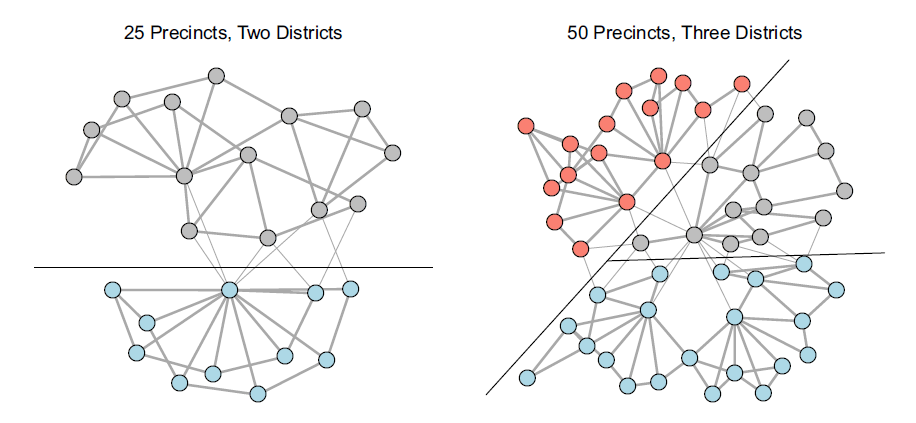
\includegraphics[width=0.8\linewidth]{img/graphcut.png}
    \label{fig:graphcut}
    \raggedright
    \figurenote{Every node is a precinct, and nodes that share an edge are known to be adjacent precincts. The algorithms "cut" edges between nodes until islands of districts are formed. \parencite[3]{fifield2020}}
\end{figure} 

\subsubsection{Sequential Monte Carlo (SMC)}
\label{sec:smc}

SMC is an implementation of the statistical method Sequential Monte Carlo\footnote{I use SMC to refer to the algorithm, not the statistical method} \parencite{mccartan2020}. The following overview provides a high-level understanding of the basic SMC algorithm.

SMC views redistricting as a graph-cutting problem, but instead of the adjacency graph, it begins with a spanning tree, a graph with the minimum number of edges to connect every node. If any edge is removed, 2 subgraphs are formed. 

\begin{figure}[hb]
    \caption{SMC Splitting Procedure}
    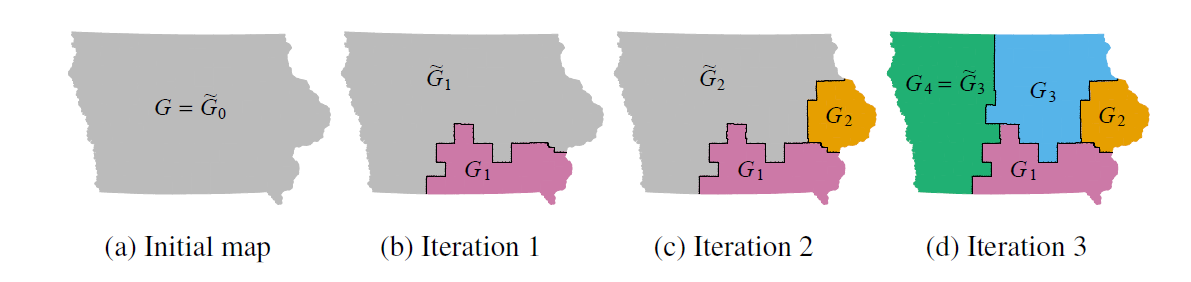
\includegraphics[width=\linewidth]{img/smc.PNG}
    \label{fig:smc}
    \raggedright
    \figurenote{One edge is chosen to be cut probabilistically, and the smaller resulting subgraph becomes a district if it meets requirements. The procedure is repeated with the remaining subgraph until the desired number of districts are formed. \parencite[14]{mccartan2020}}
\end{figure}

Figure \ref{fig:smc} visualizes the iterative splitting procedure used by SMC. First, it computes the deviation from the target precinct population for each subgraph generated by cutting each edge in the spanning tree. Then, it randomly cuts one of the edges, creating two subgraphs. If the smaller subgraph meets the population and compactness requirements, then it's accepted as the first district, and the splitting procedure is repeated with the other subgraph. This process generates the possible redistricting plans that satisfy the requirements\footnote{For more details, please refer to \textcite{mccartan2020}.}.

\subsubsection{Compact Random Seed Growth (CRSG)}
\label{sec:crsg}

The following is a high-level overview of the CRSG algorithm. For more details, please refer to \textcite[249-50]{chen2013}.

CRSG begins with declaring that every precinct is it's own district. A random precinct is then chosen, and then its geographically-closest neighbor is merged with it, creating one fewer district. This process is repeated until it arrives at the desired number of districts. \parencite[249-50]{chen2013}

After this procedure, the districts are relatively compact due to the geographic proximity requirement, but there is no guarantee that the districts are within the required population percentage of each other. To satisfy the population parity requirements, CRSG does the following. First, it identifies the two adjacent districts that have the greatest difference in total population. Then the precinct in the more populous district that is furthest from the center of said district is reassigned to the less populous district, provided that this reassignment doesn't break either district into parts. This process is repeated until all of the districts are within some desired percentage of the mean district population. \parencite[249-50]{chen2013}.

One run of CRSG will produce one set of districts, and separate runs of CRSG with the same input data may produce slightly different districts.

\subsection{Compactness Measures}

A universal requirement of districts is that they be "reasonably compact." There is no single legal nor scholarly definition of compactness \parencite{katz2020}. The following is a brief overview of several different, commonly used compactness measures that vary in approach, benefits, and weaknesses.

\subsubsection{Polsby-Popper Score}
\label{sec:polsbypopper}

\textcite{polsby1991} introduces the Polsby-Popper score first developed in paleontology to the problem of gerrymandering. It computes the ratio of the area of the district to the area of a circle with the same perimeter as the district \parencite{cox1927,polsby1991}. It ranges from 0 to 1, where 1 is most compact \parencite{polsby1991}.

Limitations and criticisms of this measure include that it is very sensitive to both geography and map resolution. Particularly near coastlines, even the most compact districts can have Polsby-Popper scores that are lower than gerrymandered districts which don't border coastlines. At finer resolutions, the same district will have a lower Polsby-Popper score as the perimeter increases. \parencite[12]{mccartan2020}.

\subsubsection{Edge-Cut Compactness}
\label{sec:edgecut}

Edge-Cut Compactness takes a graph theory perspective to district compactness. The edge-cut compactness score is the number of edges that must be "cut" from the original adjacency graph to the subgraphs (districts) \parencite{dube2016}. Theoretically, more compact districts will require fewer edges to be cut \parencite{dube2016}. When normalized to the number of edges and subtracted from 1, a score of 1 indicates the most compact district. 

Benefits of this measure include that it is unaffected by political and natural geography, map resolution, and population density \parencite[11]{mccartan2020}. 

\subsection{Partisan Fairness Measures}

The following is an overview of the partisan fairness measures in literature, as well as their merits and disadvantages. 

\subsubsection{Seats-Votes Curve}

Seats-votes curves have been used to assess district plans for more than 40 years, and they are broadly supported by the literature \parencite{katz2020}. Seats-votes curves plot the relationship between the population vote and the power balance in a legislature (or delegation). This plot has $V$, the average district-level proportion of votes won by Democrats (DVS), on the x-axis, and $S(V)$, the proportion of seats won by Democrats, on the y-axis \parencite{tufte1973}. Figure \ref{fig:seatsvotes} illustrates several hypothetical seats-votes curves.

\begin{figure}[hb]
    \caption{Types of Seats-Votes Curves}
    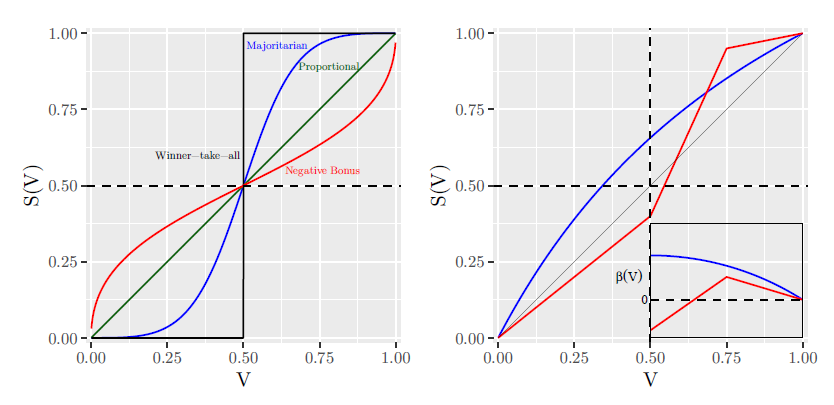
\includegraphics[width=0.8\linewidth]{img/seatsvotes.png}
    \label{fig:seatsvotes}
    \raggedright
    \figurenote{Left panel: Symmetric (fair) curves with differing levels of electoral responsiveness Right panel: Asymmetric (biased) curves, including one consistently biased toward the Democrats (blue) and one with biases favoring different parties depending on V (red); the inset graph is for (V ) for V 2 [0:5; 1] with the vertical axis scaled to be the same as the main plot, and lines color coded to the seats-votes curves. \parencite[175]{katz2020}}
\end{figure}

It's very rare to observe sufficient electoral outcomes under the same electoral system in order to plot the complete curve. (i.e., it's unlikely to observe DVS from 0 to 1 in separate elections occuring in the same districts.) In practice, one can estimate a seats-votes curve using the uniform partisan swing principle \parencite{tufte1973}.

Uniform partisan swing is the principle that, when the DVS changes by some amount between elections, the individual vote share at the district level also changes by the same amount \parencite{tufte1973}. \textcite{katz2020} empirically verified this to be true in 646 different elections. 

Thus, given a list of district-level Democratic vote proportions from one election, one can adjust each vote proportion by an arbitrarily small amount until the entire seats-votes curve is computed \parencite{katz2020}.

The benefit of seats-votes curves is that they allow a complete view of the biases of a district map across all possible average district votes \parencite{gelman1994}. Unfortunately, generating these curves for one electoral map requires the use of statistical assumptions such as uniform partisan swing, as the number of elections occurring under a since district map is usually prohibitively small \parencite{warrington2018}.

Seats-votes curve visually represent the principles of partisan symmetry and partisan bias.

\paragraph{Partisan Symmetry}

A legislature (or delegation) exhibits partisan symmetry if both parties can receive $m$ proportion of the overall votes and therefore have $n$ proportion of the seats \parencite{katz2020}. If Republicans win 60\% of the votes but control 65\% of the seats, in a symmetrical system, Democrats should also be able to control 65\% of the seats by winning 60\% of the votes. Seats-votes curves that are rotationally-symmetrical about the center exhibit partisan symmetry.

\paragraph{Partisan Bias}
\label{sec:bias}

Partisan Bias is the deviation from partisan symmetry in a tied election. If Democrats with 50\% of the average district vote but only win 40\% of the seats, there is a partisan bias of -0.1. Seats-votes curves that do not intersect the point $(0.5, 0.5)$ (the center) exhibit partisan bias.

\subsubsection{Single-Valued Fairness Measures}

The following measures compute a single number to assess the partisan fairness of a redistricting plan and are actively disputed by areas of the literature.

\paragraph{Efficiency Gap}
\label{sec:effgap}

The efficiency gap is the difference between the number of wasted votes for each party, normalized to the total number of votes, where "wasted votes" are all votes for losing candidates and all votes for winning candidates over the 50\%-plus-one threshold. Theoretically, wasted votes are a sign of "packing" or "cracking," where a gerrymandered district intentionally grouped voters together into the same district or diluted their political power across several districts. \parencite{stephanopoulos2014}

\textcite{veomett2018} found that the efficiency gap is not a measure of partisan symmetry, as the measure becomes confused in highly non-competitive elections (e.g. party wins 80\% of the vote and 100\% of the seats). 

\paragraph{Declination}
\label{sec:declination}

Declination is another proposed measure of partisan asymmetry that "...relies only on the fraction of seats each party wins in conjunction with the aggregate vote each party uses to win those seats" \parencite[3]{warrington2018}. Broadly, it measures the declination in the line connecting the average vote proportions of one party in districts controlled by the other party. See Figure \ref{fig:dec} for a visualization. 

\begin{figure}[h]
    \caption{Sample Declination Plots}
    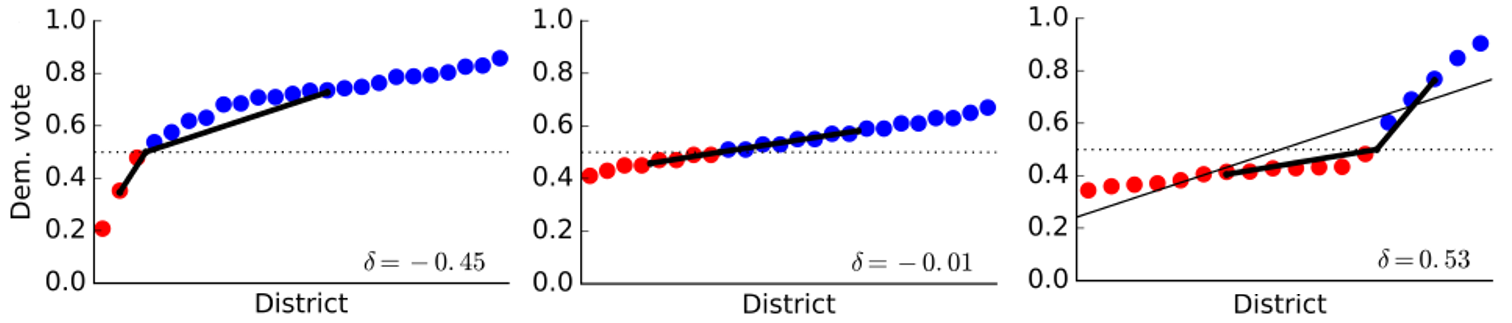
\includegraphics[width=0.8\textwidth]{img/dec.PNG}
    \label{fig:dec}
    \raggedright
    \figurenote{Districts plotted by ascending Democratic vote proportion. $\delta \approx 0$ is fair, $\delta < 0$ favors Democrats, and $\delta > 0$ favors Republicans. \parencite[6]{warrington2018}}
\end{figure}

\textcite{katz2020} refutes the claim of \textcite{warrington2018} that declination is a measure of partisan symmetry for the same reason that they refute the claim of partisan symmetry of declination, but acknowledges that it is a useful measure of the skewness of the distribution of district vote proportions. 

\subsubsection{Mean-Median Difference}
\label{sec:meanmed}

The mean-median difference is the difference between the mean and median DVS (first proposed by \textcite{mcdonald2015}). A mean-median difference of 0 indicates fair districts. 

\textcite{katz2020} finds that the mean-median difference is a reliable estimator of partisan bias only in highly competitive elections, when the average DVS is close to 0.5 \parencite[27-9]{katz2020}.
\section{Method}
\label{sec:method}

\begin{figure}
    \centering
    \caption{Project Flowchart}
    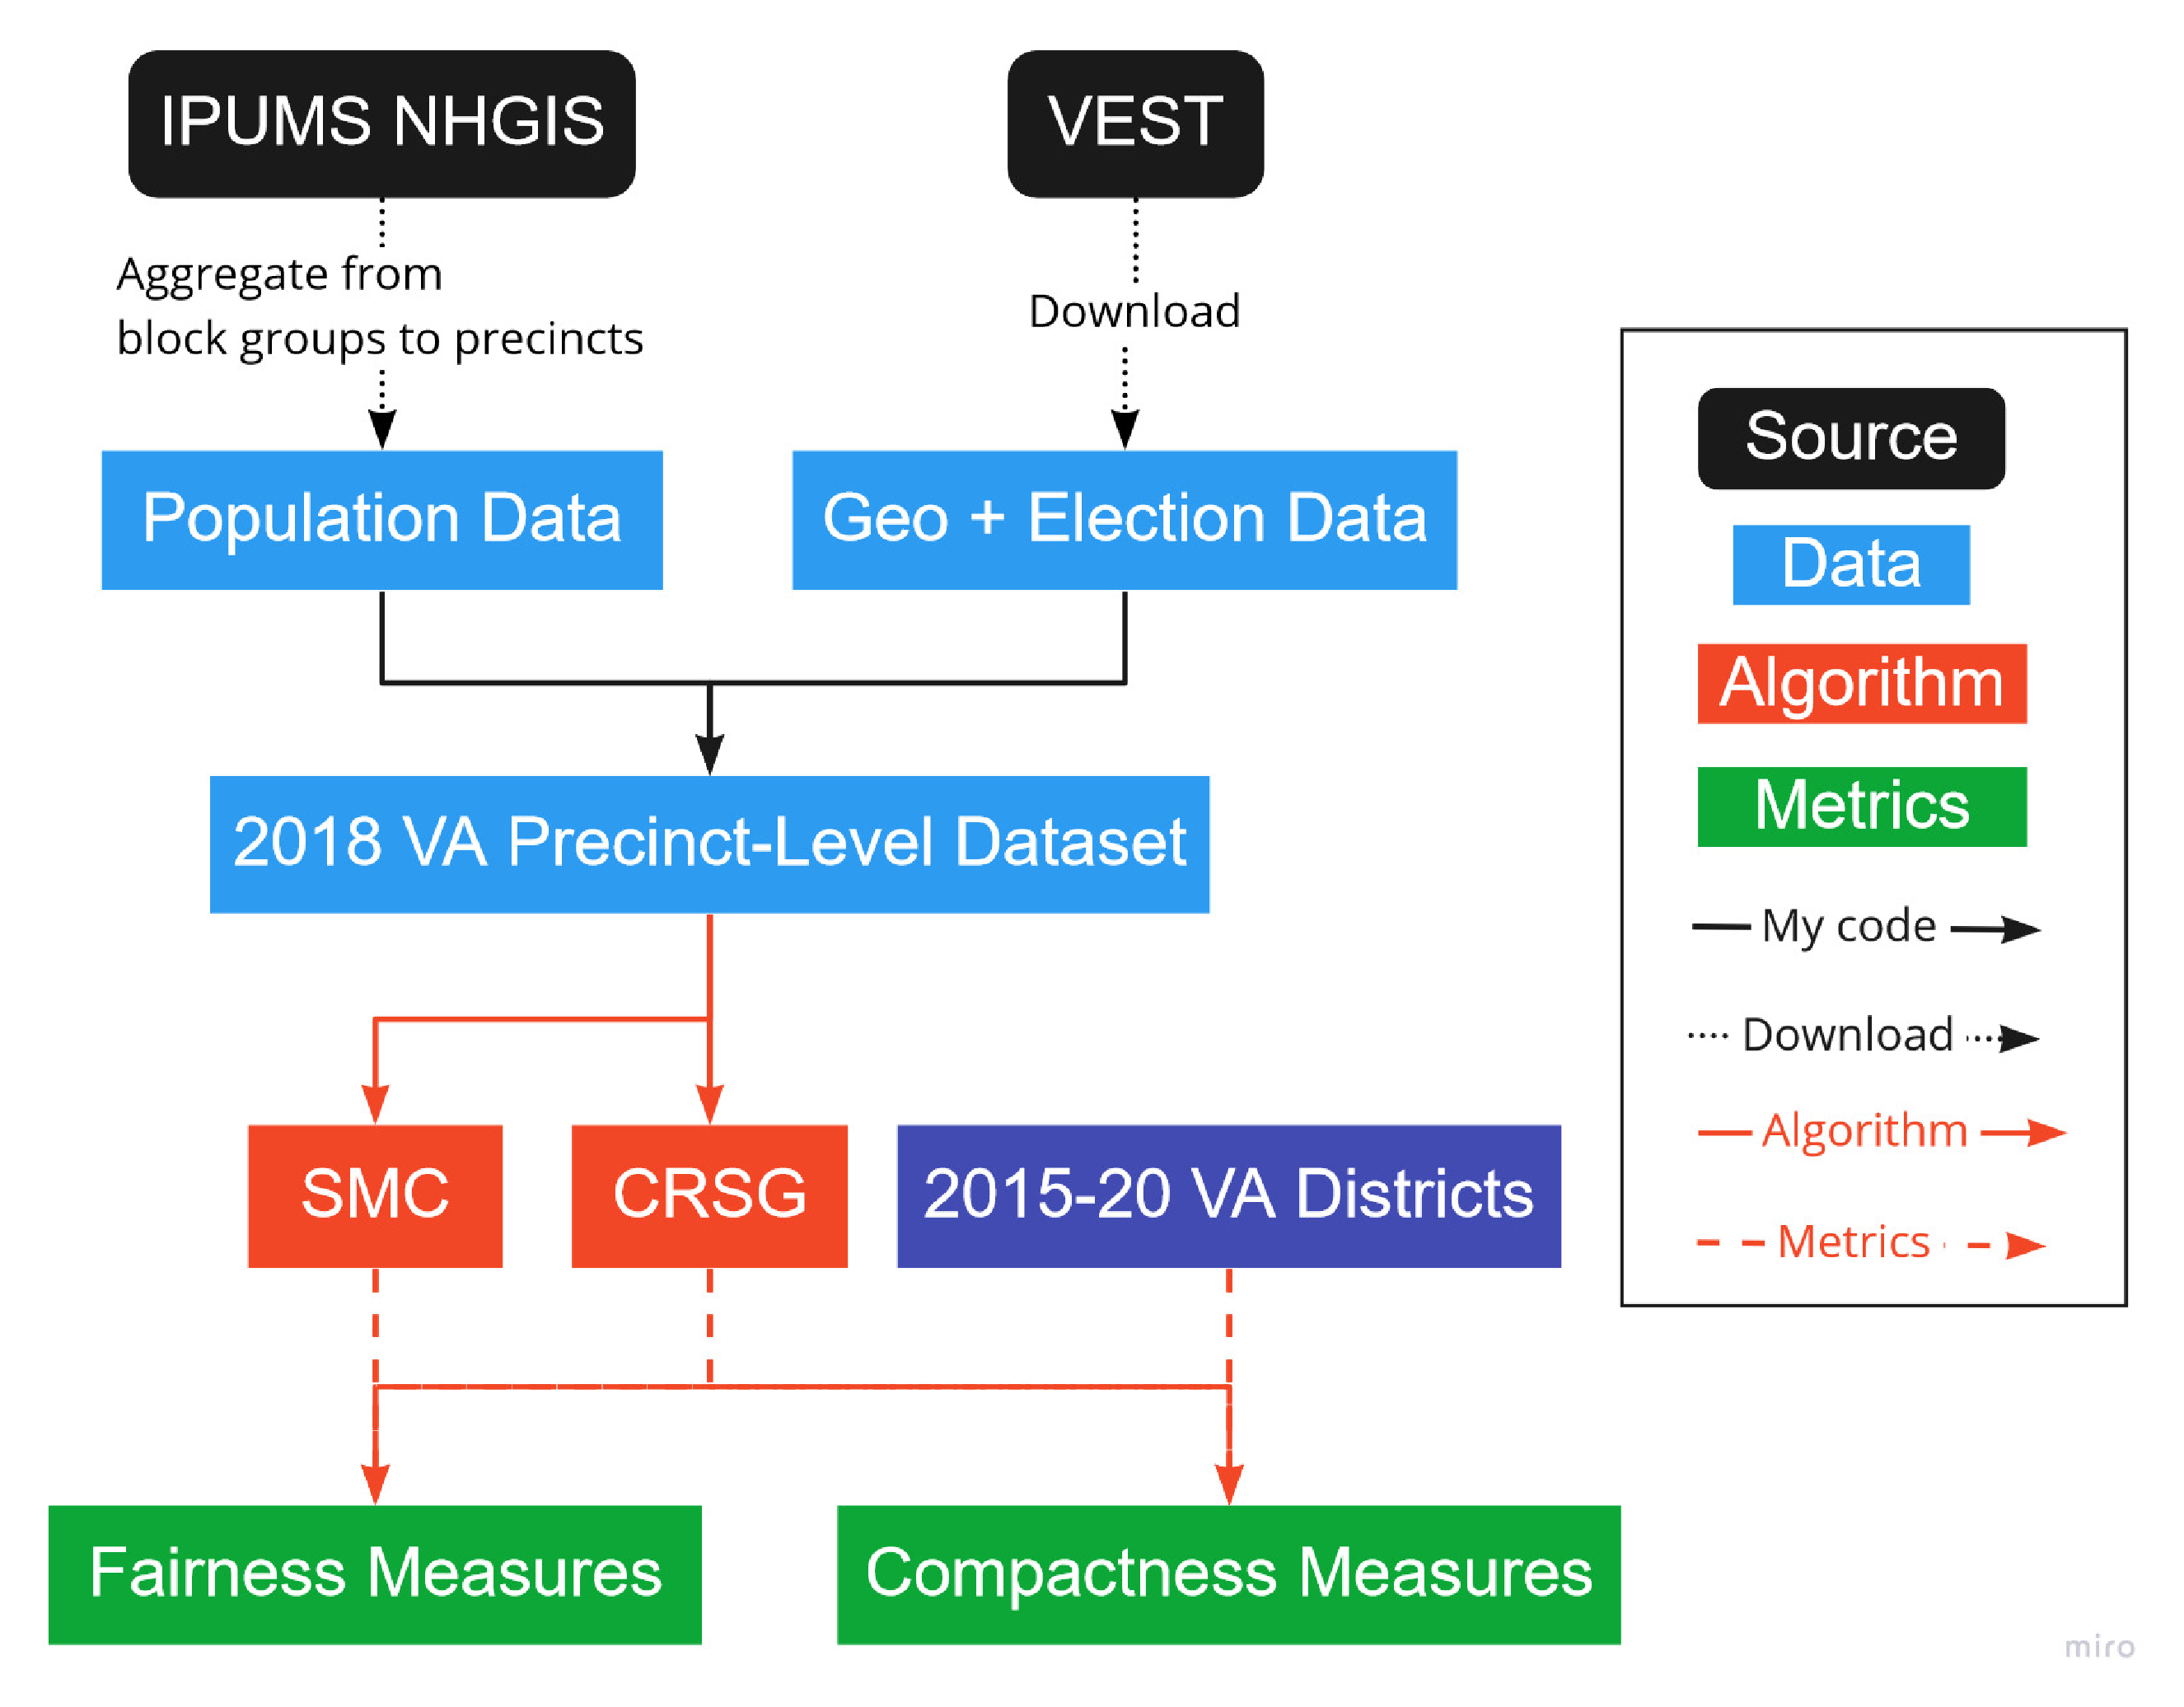
\includegraphics[width=\linewidth]{img/flowchart.pdf}
    \label{fig:flowchart}
    \raggedright
    \figurenote{Black, blue, purple, red, and green correspond to sources, data, the control, algorithms, and metrics, respectively.}
\end{figure}  

My research method simulates the 2021 redistricting of the congressional districts in Virginia using two different algorithms supplied with data from 2018. Figure \ref{fig:flowchart} provides and overview of this process.

\subsection{Choice of Research Method}

I chose the experimental design method because it allowed me to isolate the impact of the redistricting algorithm on map quality from possible confounding variables. This method also includes the use of a control group, which allows the researcher to establish causation. 

\subsection{Components of Experimental Design}

The experimental unit is the complete dataset for 2018 in Virginia. Every row in each dataset corresponds to a precinct, the smallest geographical unit by which votes are tabulated in Virginia. For each precinct, I also have the total population and the number of votes cast for the 2018 Democratic and Republican candidates. Additionally, each precinct has a polygon associated with it that represents its geographical shape.

The treatments  are the two different redistricting algorithm that I'm comparing: SMC and CRSG. I'm using the implementations in the R programming language "redist" package \parencite{fifield2020d}. The algorithms were chosen because they represent an evolution in the design of algorithms within the scholarship while still meeting the equal population and compactness requirements.

The response variables are the compactness measures and partisan fairness measures that I outlined in the literature review. This includes the Polsby-Popper score, the edge-cut compactness measure, the seats-votes curve, partisan bias, the efficiency gap, declination, and the mean-median difference. Each measure is computed for each map generated by each algorithm.

The control group is the official Virginia Congressional district map from 2015-2020. I compute the same metrics for this map as for the maps generated by the algorithms.

\subsubsection{Principles of Experimental Design}

Every experimental unit will receive each treatment, and every experimental unit can be replicated many times without issue, so there’s no error from a lack of randomization. 

Each algorithm will generate 100 sample redistricting plans. This is large enough to allow for inferences, but small enough to still be computationally feasible. 

All of the redistricting will be happening in controlled environments, so there will be no way for lurking variables to creep in and confound my results. 

\subsection{Data Cleaning}

To create my datasets, I cleaned and compiled three different types of data: demographic data, Geographic Information Systems (GIS) data, and election data.

One required piece of data in order to redistrict is demographic data at the precinct level. For my purposes, this means the total population of each precinct. To run the most accurate redistricting simulations, these data needed to be as recent as possible. Comprehensive population counts are only conducted by the US Census Bureau every 10 years, so I instead used the 5-year American Community Survey results at the block-group level. This is a sample survey, not a population count, but that is offset by the aggregation of sample data over a 5 year period. I downloaded this data from the IPUMS National Historic GIS project \parencite{mansonsteven2020}. Using the "maup" Python Library \parencite{hully}, I disaggregated the data from the block-group level to the block level, prorating the demographic data based on population. This data was then aggregated up to the precinct level, resulting in a total population count for each precinct.

To redistrict, the algorithms need to know the shape and relative location of each precinct. In practice, this means every precinct has a polygon associated with it and a Coordinate Reference System that describes where these polygons fall in space. These data tables with the geometry column are known as "shapefiles." I accessed these shapefiles from the Voting and Election Science Team on their Harvard Dataverse \parencite{votingandelectionscienceteam2019c}. I then merged in my precinct-level demographic data tables to create shapefiles with the necessary demographic data. Since election administrators are free to change the precincts between elections, precinct shapefiles are unique to both a place and a time. I therefore used shapefile data (and demographic and eleciton data) from 2018, the most recent year it was available for.

The last required data type is the count of votes for each party in each precicnt. The shapefile dataset from the Voting and Election Science Team already included this data, which was gathered from the Virginia Department of Legislative Services \parencite{votingandelectionscienceteam2019c}.
% latex table generated in R 4.0.4 by xtable 1.8-4 package
% 
\begin{table}[ht]
    \centering
    \begin{tabular}{rrrrrl}
      \hline
     & nloop & pp\_mean & fh & ecc & alg \\ 
      \hline
    1 & 1.00 & 0.19 & 1678525923965926375464.00 & 0.78 & mcmc \\ 
      2 & 2.00 & 0.18 & 1678555212992146047046.00 & 0.78 & mcmc \\ 
      3 & 3.00 & 0.18 & 1677067766242357018664.00 & 0.78 & mcmc \\ 
      4 & 4.00 & 0.18 & 1677067766242357018664.00 & 0.78 & mcmc \\ 
      5 & 5.00 & 0.18 & 1677067766242357018664.00 & 0.78 & mcmc \\ 
      6 & 6.00 & 0.18 & 1676646389617482793060.00 & 0.78 & mcmc \\ 
      7 & 7.00 & 0.19 & 1676646389617482793060.00 & 0.78 & mcmc \\ 
      8 & 8.00 & 0.19 & 1676744236050333040640.00 & 0.78 & mcmc \\ 
      9 & 9.00 & 0.19 & 1676744236050333040640.00 & 0.78 & mcmc \\ 
      10 & 10.00 & 0.18 & 1675498547325891248168.00 & 0.78 & mcmc \\ 
      11 & 1.00 & 0.18 & 2001572309073271717828.00 & 0.81 & smc \\ 
      12 & 2.00 & 0.18 & 2001572309073271717828.00 & 0.81 & smc \\ 
      13 & 3.00 & 0.16 & 2005583564208632234024.00 & 0.80 & smc \\ 
      14 & 4.00 & 0.17 & 2001561582263223189644.00 & 0.81 & smc \\ 
      15 & 5.00 & 0.17 & 2002001952518607208488.00 & 0.80 & smc \\ 
      16 & 6.00 & 0.16 & 2005583564208632234024.00 & 0.80 & smc \\ 
      17 & 7.00 & 0.17 & 2001561582263223189644.00 & 0.81 & smc \\ 
      18 & 8.00 & 0.17 & 2001561582263223189644.00 & 0.81 & smc \\ 
      19 & 9.00 & 0.15 & 2077377512332589793280.00 & 0.79 & smc \\ 
      20 & 10.00 & 0.17 & 2001561582263223189644.00 & 0.81 & smc \\ 
      21 & 1.00 & 0.19 & 1678525923965926375464.00 & 0.78 & crsg \\ 
      22 & 2.00 & 0.18 & 1962559499619963240488.00 & 0.76 & crsg \\ 
      23 & 3.00 & 0.18 & 1936322035812456726668.00 & 0.77 & crsg \\ 
      24 & 4.00 & 0.19 & 1751283151238781993060.00 & 0.80 & crsg \\ 
      25 & 5.00 & 0.15 & 1833482317459443155984.00 & 0.76 & crsg \\ 
      26 & 6.00 & 0.17 & 2690830689268182024262.00 & 0.77 & crsg \\ 
      27 & 7.00 & 0.19 & 1530762409867006443520.00 & 0.82 & crsg \\ 
      28 & 8.00 & 0.16 & 1576994186337538015202.00 & 0.77 & crsg \\ 
      29 & 9.00 & 0.18 & 1438603084253136683048.00 & 0.82 & crsg \\ 
      30 & 10.00 & 0.17 & 1616351906889106718720.00 & 0.79 & crsg \\ 
      31 & 1.00 & 0.19 & 2154162196943879274466.00 & 0.78 & control \\ 
       \hline
    \end{tabular}
    \end{table}
\section{Discussion}
\label{sec:disc}

The goal of my research is to compare two different automated redistricting algorithms in an empirical context and to evaluate the maps they generate using a variety of compactness and partisan fairness measures that exist in the literature. 

I begin by analyzing the compactness and then the partisan fairness metrics. I will end by discussing the limitations of my findings. 

\subsection{Compactness Measures}

The compactness measures are presented in Figure \ref{fig:compact.density}. 

The \hyperref[sec:polsbypopper]{Polsby-Popper score} compares the area of the district to the area of a circle with the same perimeter as the district \parencite{polsby1991}. It ranges from 0 to 1, where higher values indicate a compacter district \parencite{polsby1991}. The \hyperref[sec:smc]{SMC} maps averaged a Polsby-Popper score of $0.155$, which is slightly less compact than the existing district ($0.186$). The \hyperref[sec:crsg]{CRSG} maps also averaged a score just slightly less than the existing district ($0.179$). Through the lens of this measure, CRSG produced maps as compact as the existing map, and SMC's maps were slightly less compact, on average. 

The second compactness metric measured was the \hyperref[sec:edgecut]{edge-cut compactness measure}, a measure grounded in graph theory. It measures the proportion of edges that had to be cut from the initial precinct graph to form the districts, and it has been normalized to the total number of edges in the original adjacency graph \parencite{dube2016}. Through the lens of edge-cut compactness, SMC maps were more compact than the existing map ($0.811 > 0.777$), and CRSG maps were just as compact as existing maps ($0.778 \approx 0.777$). 

Both compactness measures did not reach the same conclusions. The Polsby-Popper score found the SMC maps to be less compact on average than the control, while the edge-cut compactness measure found the SMC maps to be more compact. This is likely because Polsby-Popper scores are very sensitive to resolution and geography \parencite{mccartan2020}. Virginia is a state with high-perimeter borders, defined by the Blue Ridge Mountains and the Chesapeake Bay \parencite{unitedstatesgeologicalsurvey2021}. Additionally, Accomack County includes the Virginia Barrier Islands, which are separately from the mainland of the state \parencite{unitedstatesgeologicalsurvey2021}. Therefore, the very uneven geographic border of Virginia likely interfered with the ability of the Polsby-Popper score to fairly quantify compactness. With that in mind, if we only consider edge-cut compactness, SMC was able to generate compacter maps than both CRSG and the existing map. However, both distributions were reasonably compact, and there are no worrying significant in compactness between the three proposals. 

\subsection{Partisan Fairness Measures}

Continuing with the partisan fairness measures, I'll first analyze the \hyperref[sec:seatsvotes]{seats-votes curves}, and then the single-valued measures outlined in the \hyperref[sec:litreview]{Literature Review}. 

\subsubsection{Seats-Votes Curves}

When viewing the seats-votes curves in Figure \ref{fig:sv} in aggregate, the 100 curves for SMC in a) form a majoritarian seats-votes curve (see Figure \ref{fig:seatsvotes}). Partisan symmetry is the rotational symmetry about the point $(0.5, 0.5)$ of this graph \parencite{katz2020}, and the SMC map curves display partisan symmetry. The same is true for the 100 curves from CRSG in b). This indicates that both algorithms generated maps that, when taken together, do not advantage one party over the other. Compared to the curve for the 2018 district map in 2018 (shown in c)), the two algorithms generated more-symmetrical maps. The existing map is still majoritarian (see Figure \ref{fig:seatsvotes}), but it favors Republicans from DVS $[0, 0.54]$ and Democrats from $[0.54, 1]$. If Democrats won 50\% of the average district vote, they'd win about 38\% of the seats, not 50\%. In summary, both algorithms generated more-symmetrical maps on average when compared to the existing map. 

\subsubsection{Single-Valued Partisan Fairness Measures}

Next I will analyze the \hyperref[sec:bias]{partisan bias}, \hyperref[sec:effgap]{the efficiency gap}, \hyperref[sec:declination]{declination}, and \hyperref[sec:meanmed]{mean-median difference} distributions for the two algorithms. These results are visualized in Figure \ref{fig:fair.density}.

Partisan bias is the deviation from partisan symmetry at an average district-level Democratic vote share (DVS) of 0.5. On a seats-votes curve (see Figure \ref{fig:sv}), this is the difference between 0.5 and the y-coordinate of the curve at $x=0.5$. As shown in a), the SMC maps, on average, were very fair ($0.00455 \approx 0$). e) shows this to be true for the CRSG maps as well, though they do slightly favor Democrats ($0.0364 > 0$). Both algorithms generated less biased maps on average than the existing maps, which significantly favored Republicans ($-0.136 < 0$). These results align with the conclusions drawn from the seats-votes curve. Interestingly, the existing map is biased towards Republicans, but this is not evident in the election map, as the actual DVS is greater than 0.5. Nevertheless, both algorithms generated less biased maps, on average, than the existing map. 

Next is the efficiency gap, which measures the difference in "wasted votes" between each party, normalized to the total vote count, and it ranges from -1 to 1 \parencite{stephanopoulos2015}. All three sets of maps; SMC, CRSG, and the existing map; have an efficiency gap within the acceptable margin ($\pm 0.08$) \parencite{stephanopoulos2015}. The efficiency gap doesn't find evidence of significant differences in the number of wasted votes between the Democratic and Republican parties between the algorithms and the existing districts. This aligns with the literature, as most criticisms of the efficiency gap point out that is mischaracterizes "wasted votes" in highly non-competitive elections (see \textcite{veomett2018} and \textcite{katz2020}). However, Virginia is a very competitive state, so this does not appear to apply here.

The next measure is declination, which quantifies the concavity of the the line on the plot of districts by ascending DVS; see Figure \ref{fig:dec} for a visualization. It ranges from -1 to 1, with values of 0 indicating fairness \parencite{warrington2018}. The SMC maps are on average fair ($0.00523 \approx 0$), as is the existing map ($0.0406 \approx 0$). However, the declination of the CRSG favors Democrats ($-0.163 < 0$). Seeing as the seats-votes curves for SMC and CRSG were found to be symmetrical, these results agree with the findings of \textcite{katz2020} that declination is not a measure of symmetry, but rather of the skewness of the district vote proportion distribution. This district-level vote proportion distribution appears to be skewed towards Democrats on average in the CRSG maps, and centered in the average SMC maps and the existing map. 

The final measure is the mean-median difference, which is the difference between the mean and median DVS. It ranges in value from -1 to 1, with values of 0 indicating a symmetrical distribution \parencite{mcdonald2015}. \textcite{katz2020} finds that at an average DVS of 0.5 (a tied election), the mean-median difference measures partisan bias. The result that the existing map slightly favors Republicans ($0.068 > 0$) while the average SMC maps and CRSG maps are essentially fair ($-0.0118 \approx 0, -0.0109 \approx 0$) aligns with the results from the partisan bias measure, which supports the findings of \textcite{katz2020}. 

When viewed together, the partisan fairness measures illustrate the following conclusions. SMC generated fair and symmetrical districts from the perspective of all four measures. CRSG also generated, on average, fair districts, with only a skew in the district-level DVS distribution. Both algorithms produced, on average, fairer districts than the existing map, which was found to be biased towards Republicans by the established partisan fairness measures (the seats-votes curve and partisan bias). 

\subsection{Limitations}

The limitations of the compactness measures derives largely from their sensitivity to geography. Additionally, the seats-votes curves are very sensitive to the idiosyncrasies of the particular election since the number of seats is so small. Each algorithm generated 100 maps, so the likelihood of randomly generating biased maps could be reduced by increasing the number of maps each algorithm generated. Finally, every district-level DVS was calculated using only the votes for the Democratic and Republican parties, ignoring third-party candidates.

\subsection{Interpretations}

There were not significant differences in the average compactness of maps generated by the algorithms and the existing map. The compactness measures provided additional evidence that the Polsby-Popper score cannot accurately measure compactness when faced with districts that have lengthy perimeters due to their geography. 

SMC was found to generate fair, symmetrical districts. CRSG districts were mostly fair, though they showed a slight Democratic bias in some cases. The control districts were found to be biased towards Republicans by all established measures of partisan fairness. 
\section{Conclusion}
\label{sec:conc}

The objective of this research was fill the gap in the scholarship with respect to comparative, empirical case studies of the performance of automated redistricting algorithms. I therefore set out to answer the question, \emph{how do the hypothetical district maps for the Virginia Congressional delegation for the 2020s generated by different automated redistricting algorithms compare based on partisan fairness and compactness measures?}

In my experimental case study, I simulated the 2021 redistricting of the congressional districts in Virginia using the CRSG and SMC algorithms, and evaluated the resulting maps and the existing map using various measures of compactness\footnote{The Polsby-Popper score and the edge-cut compactness score} and of partisan fairness\footnote{The seats-votes curve, partisan bias, the efficiency gap, declination, and the mean-median difference}. 

The key conclusions from my research are that SMC reliably generated the fairest districts, that CRSG generated fair districts less reliably, and that the existing district map significantly favored Republicans. This suggests that SMC is the favored choice of algorithm for such a redistricting task. Both algorithms and the existing map were reasonably compact.

Regarding compactness measures, I confirmed the findings of \textcite{mccartan2020} that the Polsby-Popper measure fails to assess compactness fairly when physical geography necessitates a certain degree of incompactness. I find the edge-cut compactness measure to be robust against variations in physical geography, which confirms the findings of \textcite{dube2016}.

Regarding measures of partisan fairness, the seats-votes curve provided the clearest picture of irregularities in the seats-votes relationship, which agrees with the conclusions of \textcite{katz2020}. I also find the mean-median difference to align with the partisan bias measure, as theoretically verified by \textcite{katz2020}. My results also confirmed the findings of \textcite{veomett2018} that the efficiency gap can measure partisan symmetry in competitive elections. Lastly, I also find declination to measure the skewness in the district vote distribution, not partisan fairness, confirming the theory of \textcite{katz2020}. 

Taken in concert, my findings present a significant evolution in the capabilities of automated redistricting algorithms, as well as initial evidence that the SMC algorithm could successfully be used by a redistricting commission tasked with redrawing district boundaries. Tangentially, I also provided limited empirical evidence supporting the findings of various scholars that certain measures either do or do not assess deviation from partisan symmetry.

As the SMC algorithm continues to evolve and improve, we could be approaching a reality where a number of fair redistricting maps are generated by algorithms, and then the final map is selected by members of a committee that represents various stakeholders.

However, further research is needed to continue evaluating redistricting algorithms as they continue to improve. My research only focused on a single redistricting cycle of a single delegation of a single state. Furthermore, access to greater computing power would enable the generation of larger sets of maps and for maps with more districts. Additionally, empirical evaluations of these algorithms will need to include further real-world stipulations, such as obeying county boundaries, preserving majority-minority districts, and generating districts that vary minimally from the existing districts. 

Such research will enable the transition of automated redistricting algorithms from the scholarly literature into practice in independent commissions, which is one necessary step towards the goal of increasing fairness in our district-based democracy. 

\printbibliography

\end{document}
